% Created by tikzDevice version 0.12 on 2019-01-19 16:45:03
% !TEX encoding = UTF-8 Unicode
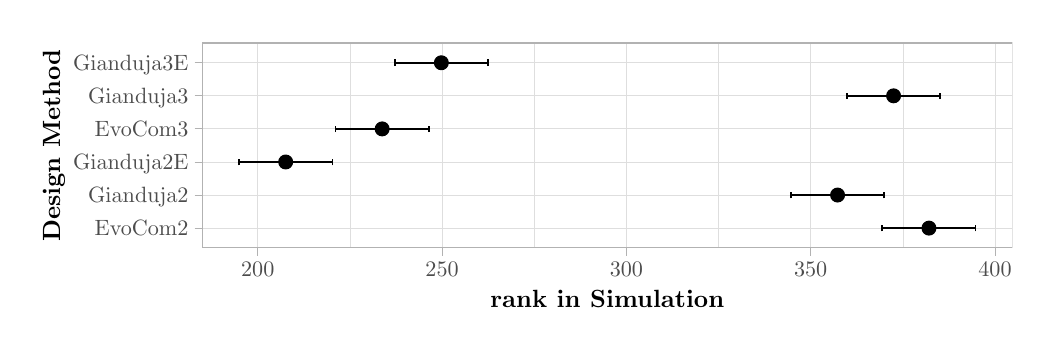
\begin{tikzpicture}[x=1pt,y=1pt]
\definecolor{fillColor}{RGB}{255,255,255}
\path[use as bounding box,fill=fillColor,fill opacity=0.00] (0,0) rectangle (361.35,108.41);
\begin{scope}
\path[clip] (  0.00,  0.00) rectangle (361.35,108.40);
\definecolor{drawColor}{RGB}{255,255,255}
\definecolor{fillColor}{RGB}{255,255,255}

\path[draw=drawColor,line width= 0.6pt,line join=round,line cap=round,fill=fillColor] (  0.00,  0.00) rectangle (361.35,108.40);
\end{scope}
\begin{scope}
\path[clip] ( 63.07, 28.81) rectangle (355.85,102.90);
\definecolor{fillColor}{RGB}{255,255,255}

\path[fill=fillColor] ( 63.07, 28.81) rectangle (355.85,102.90);
\definecolor{drawColor}{gray}{0.87}

\path[draw=drawColor,line width= 0.1pt,line join=round] (116.43, 28.81) --
	(116.43,102.90);

\path[draw=drawColor,line width= 0.1pt,line join=round] (183.04, 28.81) --
	(183.04,102.90);

\path[draw=drawColor,line width= 0.1pt,line join=round] (249.64, 28.81) --
	(249.64,102.90);

\path[draw=drawColor,line width= 0.1pt,line join=round] (316.25, 28.81) --
	(316.25,102.90);

\path[draw=drawColor,line width= 0.3pt,line join=round] ( 63.07, 35.98) --
	(355.85, 35.98);

\path[draw=drawColor,line width= 0.3pt,line join=round] ( 63.07, 47.93) --
	(355.85, 47.93);

\path[draw=drawColor,line width= 0.3pt,line join=round] ( 63.07, 59.88) --
	(355.85, 59.88);

\path[draw=drawColor,line width= 0.3pt,line join=round] ( 63.07, 71.83) --
	(355.85, 71.83);

\path[draw=drawColor,line width= 0.3pt,line join=round] ( 63.07, 83.78) --
	(355.85, 83.78);

\path[draw=drawColor,line width= 0.3pt,line join=round] ( 63.07, 95.73) --
	(355.85, 95.73);

\path[draw=drawColor,line width= 0.3pt,line join=round] ( 83.13, 28.81) --
	( 83.13,102.90);

\path[draw=drawColor,line width= 0.3pt,line join=round] (149.73, 28.81) --
	(149.73,102.90);

\path[draw=drawColor,line width= 0.3pt,line join=round] (216.34, 28.81) --
	(216.34,102.90);

\path[draw=drawColor,line width= 0.3pt,line join=round] (282.95, 28.81) --
	(282.95,102.90);

\path[draw=drawColor,line width= 0.3pt,line join=round] (349.55, 28.81) --
	(349.55,102.90);
\definecolor{drawColor}{RGB}{0,0,0}
\definecolor{fillColor}{RGB}{0,0,0}

\path[draw=drawColor,line width= 0.4pt,line join=round,line cap=round,fill=fillColor] (325.68, 35.98) circle (  2.50);

\path[draw=drawColor,line width= 0.4pt,line join=round,line cap=round,fill=fillColor] (292.65, 47.93) circle (  2.50);

\path[draw=drawColor,line width= 0.4pt,line join=round,line cap=round,fill=fillColor] ( 93.23, 59.88) circle (  2.50);

\path[draw=drawColor,line width= 0.4pt,line join=round,line cap=round,fill=fillColor] (128.09, 71.83) circle (  2.50);

\path[draw=drawColor,line width= 0.4pt,line join=round,line cap=round,fill=fillColor] (312.89, 83.78) circle (  2.50);

\path[draw=drawColor,line width= 0.4pt,line join=round,line cap=round,fill=fillColor] (149.48, 95.73) circle (  2.50);

\path[draw=drawColor,line width= 0.6pt,line join=round] (342.54, 34.78) --
	(342.54, 37.17);

\path[draw=drawColor,line width= 0.6pt,line join=round] (342.54, 35.98) --
	(308.82, 35.98);

\path[draw=drawColor,line width= 0.6pt,line join=round] (308.82, 34.78) --
	(308.82, 37.17);

\path[draw=drawColor,line width= 0.6pt,line join=round] (309.51, 46.74) --
	(309.51, 49.13);

\path[draw=drawColor,line width= 0.6pt,line join=round] (309.51, 47.93) --
	(275.80, 47.93);

\path[draw=drawColor,line width= 0.6pt,line join=round] (275.80, 46.74) --
	(275.80, 49.13);

\path[draw=drawColor,line width= 0.6pt,line join=round] (110.09, 58.69) --
	(110.09, 61.08);

\path[draw=drawColor,line width= 0.6pt,line join=round] (110.09, 59.88) --
	( 76.38, 59.88);

\path[draw=drawColor,line width= 0.6pt,line join=round] ( 76.38, 58.69) --
	( 76.38, 61.08);

\path[draw=drawColor,line width= 0.6pt,line join=round] (144.95, 70.64) --
	(144.95, 73.03);

\path[draw=drawColor,line width= 0.6pt,line join=round] (144.95, 71.83) --
	(111.24, 71.83);

\path[draw=drawColor,line width= 0.6pt,line join=round] (111.24, 70.64) --
	(111.24, 73.03);

\path[draw=drawColor,line width= 0.6pt,line join=round] (329.75, 82.59) --
	(329.75, 84.98);

\path[draw=drawColor,line width= 0.6pt,line join=round] (329.75, 83.78) --
	(296.03, 83.78);

\path[draw=drawColor,line width= 0.6pt,line join=round] (296.03, 82.59) --
	(296.03, 84.98);

\path[draw=drawColor,line width= 0.6pt,line join=round] (166.34, 94.54) --
	(166.34, 96.93);

\path[draw=drawColor,line width= 0.6pt,line join=round] (166.34, 95.73) --
	(132.62, 95.73);

\path[draw=drawColor,line width= 0.6pt,line join=round] (132.62, 94.54) --
	(132.62, 96.93);
\definecolor{drawColor}{gray}{0.70}

\path[draw=drawColor,line width= 0.6pt,line join=round,line cap=round] ( 63.07, 28.81) rectangle (355.85,102.90);
\end{scope}
\begin{scope}
\path[clip] (  0.00,  0.00) rectangle (361.35,108.41);
\definecolor{drawColor}{gray}{0.30}

\node[text=drawColor,anchor=base east,inner sep=0pt, outer sep=0pt, scale=  0.80] at ( 58.12, 33.22) {EvoCom2};

\node[text=drawColor,anchor=base east,inner sep=0pt, outer sep=0pt, scale=  0.80] at ( 58.12, 45.18) {Gianduja2};

\node[text=drawColor,anchor=base east,inner sep=0pt, outer sep=0pt, scale=  0.80] at ( 58.12, 57.13) {Gianduja2E};

\node[text=drawColor,anchor=base east,inner sep=0pt, outer sep=0pt, scale=  0.80] at ( 58.12, 69.08) {EvoCom3};

\node[text=drawColor,anchor=base east,inner sep=0pt, outer sep=0pt, scale=  0.80] at ( 58.12, 81.03) {Gianduja3};

\node[text=drawColor,anchor=base east,inner sep=0pt, outer sep=0pt, scale=  0.80] at ( 58.12, 92.98) {Gianduja3E};
\end{scope}
\begin{scope}
\path[clip] (  0.00,  0.00) rectangle (361.35,108.41);
\definecolor{drawColor}{gray}{0.70}

\path[draw=drawColor,line width= 0.3pt,line join=round] ( 60.32, 35.98) --
	( 63.07, 35.98);

\path[draw=drawColor,line width= 0.3pt,line join=round] ( 60.32, 47.93) --
	( 63.07, 47.93);

\path[draw=drawColor,line width= 0.3pt,line join=round] ( 60.32, 59.88) --
	( 63.07, 59.88);

\path[draw=drawColor,line width= 0.3pt,line join=round] ( 60.32, 71.83) --
	( 63.07, 71.83);

\path[draw=drawColor,line width= 0.3pt,line join=round] ( 60.32, 83.78) --
	( 63.07, 83.78);

\path[draw=drawColor,line width= 0.3pt,line join=round] ( 60.32, 95.73) --
	( 63.07, 95.73);
\end{scope}
\begin{scope}
\path[clip] (  0.00,  0.00) rectangle (361.35,108.41);
\definecolor{drawColor}{gray}{0.70}

\path[draw=drawColor,line width= 0.3pt,line join=round] ( 83.13, 26.06) --
	( 83.13, 28.81);

\path[draw=drawColor,line width= 0.3pt,line join=round] (149.73, 26.06) --
	(149.73, 28.81);

\path[draw=drawColor,line width= 0.3pt,line join=round] (216.34, 26.06) --
	(216.34, 28.81);

\path[draw=drawColor,line width= 0.3pt,line join=round] (282.95, 26.06) --
	(282.95, 28.81);

\path[draw=drawColor,line width= 0.3pt,line join=round] (349.55, 26.06) --
	(349.55, 28.81);
\end{scope}
\begin{scope}
\path[clip] (  0.00,  0.00) rectangle (361.35,108.41);
\definecolor{drawColor}{gray}{0.30}

\node[text=drawColor,anchor=base,inner sep=0pt, outer sep=0pt, scale=  0.80] at ( 83.13, 18.35) {200};

\node[text=drawColor,anchor=base,inner sep=0pt, outer sep=0pt, scale=  0.80] at (149.73, 18.35) {250};

\node[text=drawColor,anchor=base,inner sep=0pt, outer sep=0pt, scale=  0.80] at (216.34, 18.35) {300};

\node[text=drawColor,anchor=base,inner sep=0pt, outer sep=0pt, scale=  0.80] at (282.95, 18.35) {350};

\node[text=drawColor,anchor=base,inner sep=0pt, outer sep=0pt, scale=  0.80] at (349.55, 18.35) {400};
\end{scope}
\begin{scope}
\path[clip] (  0.00,  0.00) rectangle (361.35,108.41);
\definecolor{drawColor}{RGB}{0,0,0}

\node[text=drawColor,anchor=base,inner sep=0pt, outer sep=0pt, scale=  0.90] at (209.46,  7.44) {\bfseries rank in Simulation};
\end{scope}
\begin{scope}
\path[clip] (  0.00,  0.00) rectangle (361.35,108.41);
\definecolor{drawColor}{RGB}{0,0,0}

\node[text=drawColor,rotate= 90.00,anchor=base,inner sep=0pt, outer sep=0pt, scale=  0.90] at ( 11.71, 65.86) {\bfseries Design Method};
\end{scope}
\end{tikzpicture}
